% Free-body diagram and hand-calculation sheet (\input by regrasp_pulse_math.tex)
\section{Free-body diagram and hand calculation}\label{sec:fbd}
This section contains everything needed to redo the result by hand: the forces on the block, the equation of
motion in both frames, and a phase-by-phase calculation with numbers. Symbols:
$m=0.035$\,kg, $g=9.81$\,m/s$^2$, tilt $\theta$, friction $\mu$, speed limit $V$, braking/reversing accelerations
$A_{\rm b}$, $A_{\rm r}$, and free time $T$. $\hat z$ is the grasp axis (positive up the axis) and $\hat x$ is
perpendicular to it in the tilt plane, pointing away from the lower finger.

\begin{figure}[h]
\centering
\resizebox{\linewidth}{!}{%
\begin{tikzpicture}[>=Stealth, every node/.style={font=\small}]
  % ================= (a) gripped =================
  \begin{scope}
    \node[font=\normalsize\bfseries] at (0,4.3) {(a) gripped, $t<0$};
    \draw[densely dotted, gray] (0,-3.4) -- (0,3.6);
    \node[gray] at (0.25,3.8) {vertical};
    \begin{scope}[rotate=35]
      \draw[->, gray] (0,-3.6) -- (0,3.6) node[left, text=black]{$+\hat z$};
      \fill[gray!40] (-1.15,-1.3) rectangle (-0.7,1.4);
      \fill[gray!40] (0.7,-1.3) rectangle (1.15,1.4);
      \filldraw[fill=blue!8, draw=blue!60!black, thick] (-0.7,-2.4) rectangle (0.7,2.4);
      \draw[->, very thick, green!45!black] (-2.4,0.6) -- (-0.7,0.6);
      \node[green!45!black] at (-2.75,0.6) {$N_L$};
      \draw[->, very thick, green!45!black] (2.4,0.6) -- (0.7,0.6);
      \node[green!45!black] at (2.75,0.6) {$N_R$};
      \draw[->, very thick, red!70!black] (-0.9,-1.0) -- (-0.9,0.2);
      \node[red!70!black] at (-1.45,-0.4) {$f_L$};
      \draw[->, very thick, red!70!black] (0.9,-1.0) -- (0.9,0.2);
      \node[red!70!black] at (1.45,-0.4) {$f_R$};
      \draw[->, very thick, orange!85!black] (0.25,0.9) -- (0.25,2.1);
      \node[orange!85!black] at (-0.25,1.75) {$a_g$};
    \end{scope}
    \draw[->, very thick] (0,0) -- (0,-1.7) node[right]{$mg$};
    \fill (0,0) circle (1.5pt);
    \draw[gray] (0,3.0) arc (90:125:3.0);
    \node[gray] at ({3.3*cos(107)},{3.3*sin(107)}) {$\theta$};
  \end{scope}
  % ================= (b) open =================
  \begin{scope}[shift={(9,0)}]
    \node[font=\normalsize\bfseries] at (0,4.3) {(b) fingers open, $0<t<T$};
    \draw[densely dotted, gray] (0,-3.4) -- (0,3.6);
    \node[gray] at (0.25,3.8) {vertical};
    \begin{scope}[rotate=35]
      \draw[->, gray] (0,-3.6) -- (0,3.6) node[left, text=black]{$+\hat z$};
      \draw[->, gray] (0.9,-3.2) -- (2.0,-3.2) node[right, text=black]{$+\hat x$};
      \fill[gray!40] (-1.15,-1.3) rectangle (-0.7,1.4);            % lower finger (contact)
      \fill[gray!40] (0.95,-1.3) rectangle (1.4,1.4);              % upper finger (gap exaggerated)
      \draw[->, thick, purple] (1.8,1.0) -- (1.8,-0.6);
      \node[purple] at (2.55,0.2) {$a_g=-A$};
      \filldraw[fill=blue!8, draw=blue!60!black, thick] (-0.7,-2.4) rectangle (0.7,2.4);
      % normal
      \draw[->, very thick, green!45!black] (-2.5,1.15) -- (-0.7,1.15);
      \node[green!45!black] at (-2.85,1.15) {$N$};
      % kinetic friction (u > 0)
      \draw[->, very thick, red!70!black] (-0.9,0.3) -- (-0.9,-0.9);
      \node[red!70!black] at (-1.5,-0.35) {$\mu N$};
      % gravity components
      \draw[->, dashed, thick] (0,0) -- (0,-1.64);
      \node at (0.95,-1.45) {$mg\cos\theta$};
      \draw[->, dashed, thick] (0,0) -- (-1.15*0.6,0);
      \node[fill=blue!8, inner sep=1pt] at (-0.15,0.55) {\footnotesize$mg\sin\theta$};
      % inertial force (gripper frame)
      \draw[->, very thick, dashed, orange!85!black] (0.3,0.35) -- (0.3,2.2);
      \node[orange!85!black, fill=blue!8, inner sep=1pt] at (-0.2,1.45) {\footnotesize$-m a_g$};
    \end{scope}
    \draw[->, very thick] (0,0) -- (0,-1.7) node[right]{$mg$};
    \fill (0,0) circle (1.5pt);
    \draw[gray] (0,3.0) arc (90:125:3.0);
    \node[gray] at ({3.3*cos(107)},{3.3*sin(107)}) {$\theta$};
  \end{scope}
\end{tikzpicture}}
\caption{Forces on the block (grey: finger pads; the grasp axis $+\hat z$ is tilted $\theta$ from vertical).
(a) Gripped: squeeze normals $N_L,N_R$ and static friction $f_L,f_R$ on both faces; the block moves with the gripper
acceleration $a_g$. (b) Fingers open: the block leans on the lower finger, which pushes back with normal $N$. Kinetic
friction $\mu N$ opposes the relative sliding. It is drawn for the block sliding \emph{up} the fingers ($u>0$), and it
points up the axis once the block slides back down. Dashed black: the components of $mg$. Dashed orange: the inertial
force $-ma_g$, which only appears when you write the equations in the gripper frame. The 1\,mm gap to the upper
finger is exaggerated.}
\label{fig:fbd}
\end{figure}

\subsection*{Forces while the fingers are open (b)}
There is no acceleration across the axis (the transverse controller holds the line), so the $\hat x$ balance gives
the normal load. The $\hat z$ balance then gives the motion.
\begin{center}
\small
\begin{tabular}{llll}
\toprule
Force & direction & magnitude & value at $45^\circ$, $\mu=0.05$\\
\midrule
weight $mg$ & world down & $mg$ & 0.3434 N\\
\quad along axis & $-\hat z$ & $mg\cos\theta$ & 0.2428 N\\
\quad across axis & $-\hat x$ (into lower finger) & $mg\sin\theta$ & 0.2428 N\\
normal $N$ & $+\hat x$ & $N=mg\sin\theta$ & 0.2428 N\\
friction & $-\sgn(u)\,\hat z$ & $\mu N=\mu mg\sin\theta$ & 0.01214 N\\
inertial (gripper frame only) & $-a_g$ direction & $m|a_g|$ & $0.525$ N at $A=15$\\
\bottomrule
\end{tabular}
\end{center}
\begin{align*}
  \text{across the axis:}\quad & N - mg\sin\theta = 0 \ \Rightarrow\ N=mg\sin\theta,\\[2pt]
  \text{along, world frame:}\quad & m\,\ddot z_b = -mg\cos\theta - \mu N\,\sgn(u),\\
  & \ddot z_b=-b=-g(\cos\theta+\mu\sin\theta)\ \ \text{if } u>0\ \text{(block sliding up the fingers)},\\
  & \ddot z_b=-d=-g(\cos\theta-\mu\sin\theta)\ \ \text{if } u<0\ \text{(sliding back down)},\\[2pt]
  \text{along, gripper frame:}\quad & m\,\ddot s = -mg\cos\theta - \mu N\,\sgn(u) - m a_g,\\
  & \ddot s = -a_g - b\ \ (u>0),\qquad \ddot s=-a_g-d\ \ (u<0).
\end{align*}
The displacement you want is always
\[
  s(T)=\Delta z_b-\Delta z_g=\int_0^T\big(v_b(t)-v_g(t)\big)\,dt
  \qquad\text{(area between the block and gripper velocity lines).}
\]
\emph{Stick check:} if $u=0$, the block stays put as long as $|{-a_g}-g\cos\theta|\le\mu g\sin\theta$.

\subsection*{Forces while gripped (a)}
The block has the gripper's acceleration $a_g$. Along the axis
$f_L+f_R=m(g\cos\theta+a_g)$ and across $N_L-N_R=mg\sin\theta$. Static friction must not slip,
$f_L+f_R\le\mu(N_L+N_R)\approx2\mu N_{\rm grip}$. The worst case is the pre-release acceleration up to $+V$ at
$a_g=+A$:
\[
  N_{\rm grip}\ \ge\ \frac{m\,(g\cos\theta+A)}{2\mu}\;=\;7.68\ \text{N}\ (A=15),\qquad 9.43\ \text{N}\ (A=20)
  \qquad(45^\circ,\ \mu=0.05).
\]

\subsection*{Step-by-step calculation}
Take the gripper profile of Section~\ref{sec:closed}. At release the gripper moves up at $+V$. It brakes to 0 at
$-A_{\rm b}$, reverses to $-V$ at $-A_{\rm r}$, then coasts. The block keeps sliding up the fingers ($u>0$) until
$t_p$, so its world acceleration is the constant $-b$ until then.
\begin{center}
\small
\renewcommand{\arraystretch}{1.25}
\begin{tabular}{p{3.2cm}p{6.1cm}rr}
\toprule
Step & formula & $A=15$ & $A=20$\\
\midrule
0. constants & $b=g(\cos\theta+\mu\sin\theta)$ [m/s$^2$] & 7.2836 & 7.2836\\
 & $d=g(\cos\theta-\mu\sin\theta)$ [m/s$^2$] & 6.5899 & 6.5899\\
1. braking $+V\to0$ & $t_a=V/A_{\rm b}$ & 30.000 ms & 22.500 ms\\
 & $\ddot s=A_{\rm b}-b$ [m/s$^2$] & 7.7164 & 12.7164\\
 & $u_1=(A_{\rm b}-b)t_a$ & 0.23149 m/s & 0.28612 m/s\\
 & $s_1=\tfrac12(A_{\rm b}-b)t_a^2$ & 3.4724 mm & 3.2189 mm\\
2. reversing $0\to-V$ & $t_r=V/A_{\rm r}$, \ $\ddot s=A_{\rm r}-b$ & 30.000 ms & 22.500 ms\\
 & $u_2=u_1+(A_{\rm r}-b)t_r$ & 0.46299 m/s & 0.57224 m/s\\
 & $s_2=s_1+u_1t_r+\tfrac12(A_{\rm r}-b)t_r^2$ & 13.8896 mm & 12.8754 mm\\
3. coast to the peak & $\ddot s=-b$, \ $t_s=u_2/b$ & 63.566 ms & 78.566 ms\\
 & $t_p=t_a+t_r+t_s$ \ (must be $<T$) & 123.566 ms & 123.566 ms\\
 & $s_p=s_2+u_2^2/(2b)$ & 28.6047 mm & 35.3547 mm\\
4. fall back & $r=T-t_p$, \ $\ddot s=-d$ & 1.4339 ms & 1.4339 ms\\
 & $\tfrac12 d\,r^2$ & 0.0068 mm & 0.0068 mm\\
\midrule
\textbf{result} & $s(T)=s_p-\tfrac12 d r^2$ & \textbf{28.598 mm} & \textbf{35.348 mm}\\
\bottomrule
\end{tabular}
\end{center}
If $t_p\ge T$, stop at step 3 with $s(T)=s_2+u_2(T-t_a-t_r)-\tfrac12 b(T-t_a-t_r)^2$. If $d\le0$, skip step 4,
because the block sticks at the peak.

\paragraph{Cross-check in the world frame.} Compute the two displacements separately and subtract.
The gripper covers a triangle during braking, a triangle during reversing, and a rectangle while coasting:
\[
  \Delta z_g = \tfrac12Vt_a-\tfrac12Vt_r-V(T-t_a-t_r) = -VT+\frac{3V^2}{2A_{\rm b}}+\frac{V^2}{2A_{\rm r}} .
\]
The block decelerates at $b$ from $+V$ to $-V$ until $t_p$, then at $d$:
\[
  \Delta z_b = \big(Vt_p-\tfrac12 b\,t_p^2\big)-\big(Vr+\tfrac12 d\,r^2\big),\qquad s(T)=\Delta z_b-\Delta z_g .
\]
\begin{center}
\small
\begin{tabular}{lrr}
\toprule
 & $A=15$ & $A=20$\\
\midrule
$\Delta z_g$ (gripper) & $-29.250$ mm & $-36.000$ mm\\
$\Delta z_b$ (block) & $-0.652$ mm & $-0.652$ mm\\
$s(T)=\Delta z_b-\Delta z_g$ & 28.598 mm & 35.348 mm\\
\bottomrule
\end{tabular}
\end{center}
Once released, the block moves the same way for every $A$: it goes up, comes back, and ends 0.65\,mm below where it
was released. The regrasp comes \emph{entirely} from how far the gripper travels down in the same time.

\begin{figure}[h]
\centering
\begin{tikzpicture}[>=Stealth, x=0.105cm, y=4.2cm, every node/.style={font=\small}]
  % axes
  \draw[->] (0,0) -- (132,0) node[right]{$t$ [ms]};
  \draw[->] (0,-0.58) -- (0,0.6) node[above]{$v$ [m/s]};
  \foreach \t in {0,30} \draw (\t,0.015) -- (\t,-0.015) node[below=1pt, fill=white, inner sep=1pt]{\scriptsize\t};
  \foreach \v in {-0.45,0.45} \draw (1,\v) -- (-1,\v) node[left]{\scriptsize$\v$};
  % shaded area = s
  \fill[blue!15] (0,0.45) -- (123.566,-0.45) -- (60,-0.45) -- cycle;
  \fill[red!20] (123.566,-0.45) -- (125,-0.4594) -- (125,-0.45) -- cycle;
  % gripper velocity
  \draw[very thick, blue!70!black] (0,0.45) -- (60,-0.45) -- (125,-0.45);
  \node[blue!70!black, anchor=west] at (61,-0.52) {gripper $v_g$ (slope $-A$)};
  % block velocity
  \draw[very thick, orange!85!black] (0,0.45) -- (123.566,-0.45) -- (125,-0.4594);
  \node[orange!85!black, anchor=south west, rotate=-17] at (18,0.34) {block $v_b$ (slope $-b$)};
  % markers
  \draw[dashed, gray] (60,-0.45) -- (60,0);
  \node[anchor=north east, fill=white, inner sep=1pt] at (59.5,-0.1) {$t_{\rm ramp}=2V/A=60$};
  \draw[dashed, gray] (123.566,-0.45) -- (123.566,0.2);
  \node[anchor=south east] at (123.2,0.2) {$t_p=2V/b=123.6$};
  \draw[dashed, gray] (125,-0.46) -- (125,0.2);
  \node[anchor=south west] at (125.4,0.2) {$T=125$};
  \node[blue!60!black] at (82,-0.36) {area $=s_p$};
\end{tikzpicture}
\caption{Velocities along the axis for $A_{\rm b}=A_{\rm r}=15$ (the $\theta=45^\circ$, $\mu=0.05$ example). The
relative displacement is the area between the block and the gripper lines. Up to the peak this area is a triangle
with height $2V$ and base $t_p-t_{\rm ramp}$, so $s_p=V(t_p-t_{\rm ramp})=0.45\times(123.566-60)$\,ms $=28.605$\,mm.
The tiny red sliver after $t_p$ is the fall-back, $0.007$\,mm. A larger $A$ makes the ramp steeper and the triangle
wider; $t_p$ does not move.}
\label{fig:vel}
\end{figure}

\paragraph{Quick formulas to check against.}
\begin{gather*}
  t_p=\frac{2V}{b},\qquad
  s(T)=\frac{2V^2}{b}-\frac{3V^2}{2A_{\rm b}}-\frac{V^2}{2A_{\rm r}}-\tfrac12 d\,(T-t_p)^2,\\
  \text{equal limits } A_{\rm b}=A_{\rm r}=A:\quad s(T)=V\Big(\frac{2V}{b}-\frac{2V}{A}\Big)-\tfrac12 d\,(T-t_p)^2 .
\end{gather*}

\paragraph{Where the pulse fires in the env.}
Figure~\ref{fig:timeline} places the example on the env's 20\,ms control grid.
\begin{itemize}
  \item The policy \emph{triggers} the pulse at step $k$ by moving the finger action through the midpoint.
  \item Steps $k$ and $k+1$ are the 40\,ms delay, during which the policy's own finger command applies.
  \item Steps $k+2$ to $k+7$ force the fingers fully open (120\,ms), and step $k+8$ forces them closed.
\end{itemize}
The block only comes loose once a finger opens past the block's half width (12.5\,mm of the 13\,mm stroke), so in
practice that is when the forced-open window starts. Your $T=125$\,ms free time matches this: 120\,ms forced open
plus about 5\,ms for the fingers to close back onto the block. \textbf{Assumption:} the release is at the start of
step $k+2$ and the policy does not command fully open during the delay. If it does, the block is released up to
40\,ms earlier and the free time grows to about 165\,ms.

The gripper velocity targets that realise the optimum, one per 20\,ms step ($\Delta v\le A\cdot20$\,ms $=0.3$\,m/s):
\begin{center}
\small
\resizebox{\linewidth}{!}{%
\begin{tabular}{l|ccccccccccc}
\toprule
step & $k-2$ & $k-1$ & $k$ & $k+1$ & $k+2$ & $k+3$ & $k+4$ & $k+5\dots k+7$ & $k+8$ & $k+9$ & $k+10$\\
\midrule
$v$ target [m/s] (end of step) & 0.30 & 0.45 & 0.45 & 0.45 & 0.15 & $-0.15$ & $-0.45$ & $-0.45$ & $-0.45$ & $-0.15$ & 0\\
fingers & \multicolumn{2}{c}{gripped} & \multicolumn{2}{c}{delay} & \multicolumn{5}{c}{open (block free)} & \multicolumn{2}{c}{gripped}\\
\bottomrule
\end{tabular}}
\end{center}
The gripper is at $+V$ \emph{before} the trigger, holds it through the delay, and starts braking on exactly the step
where the fingers let go. The brake takes 3 steps ($+0.45\to0.15\to-0.15\to-0.45$). The gripper then coasts at $-V$
until the block is re-gripped, and only then decelerates to rest. Timing matters: starting the brake one step
(20\,ms) \emph{early}, while the block is still gripped, drops $s(T)$ from 28.6 to 6.7\,mm. Starting it one step
\emph{late} drops it to 13.2\,mm.

\begin{figure}[h]
  \centering
  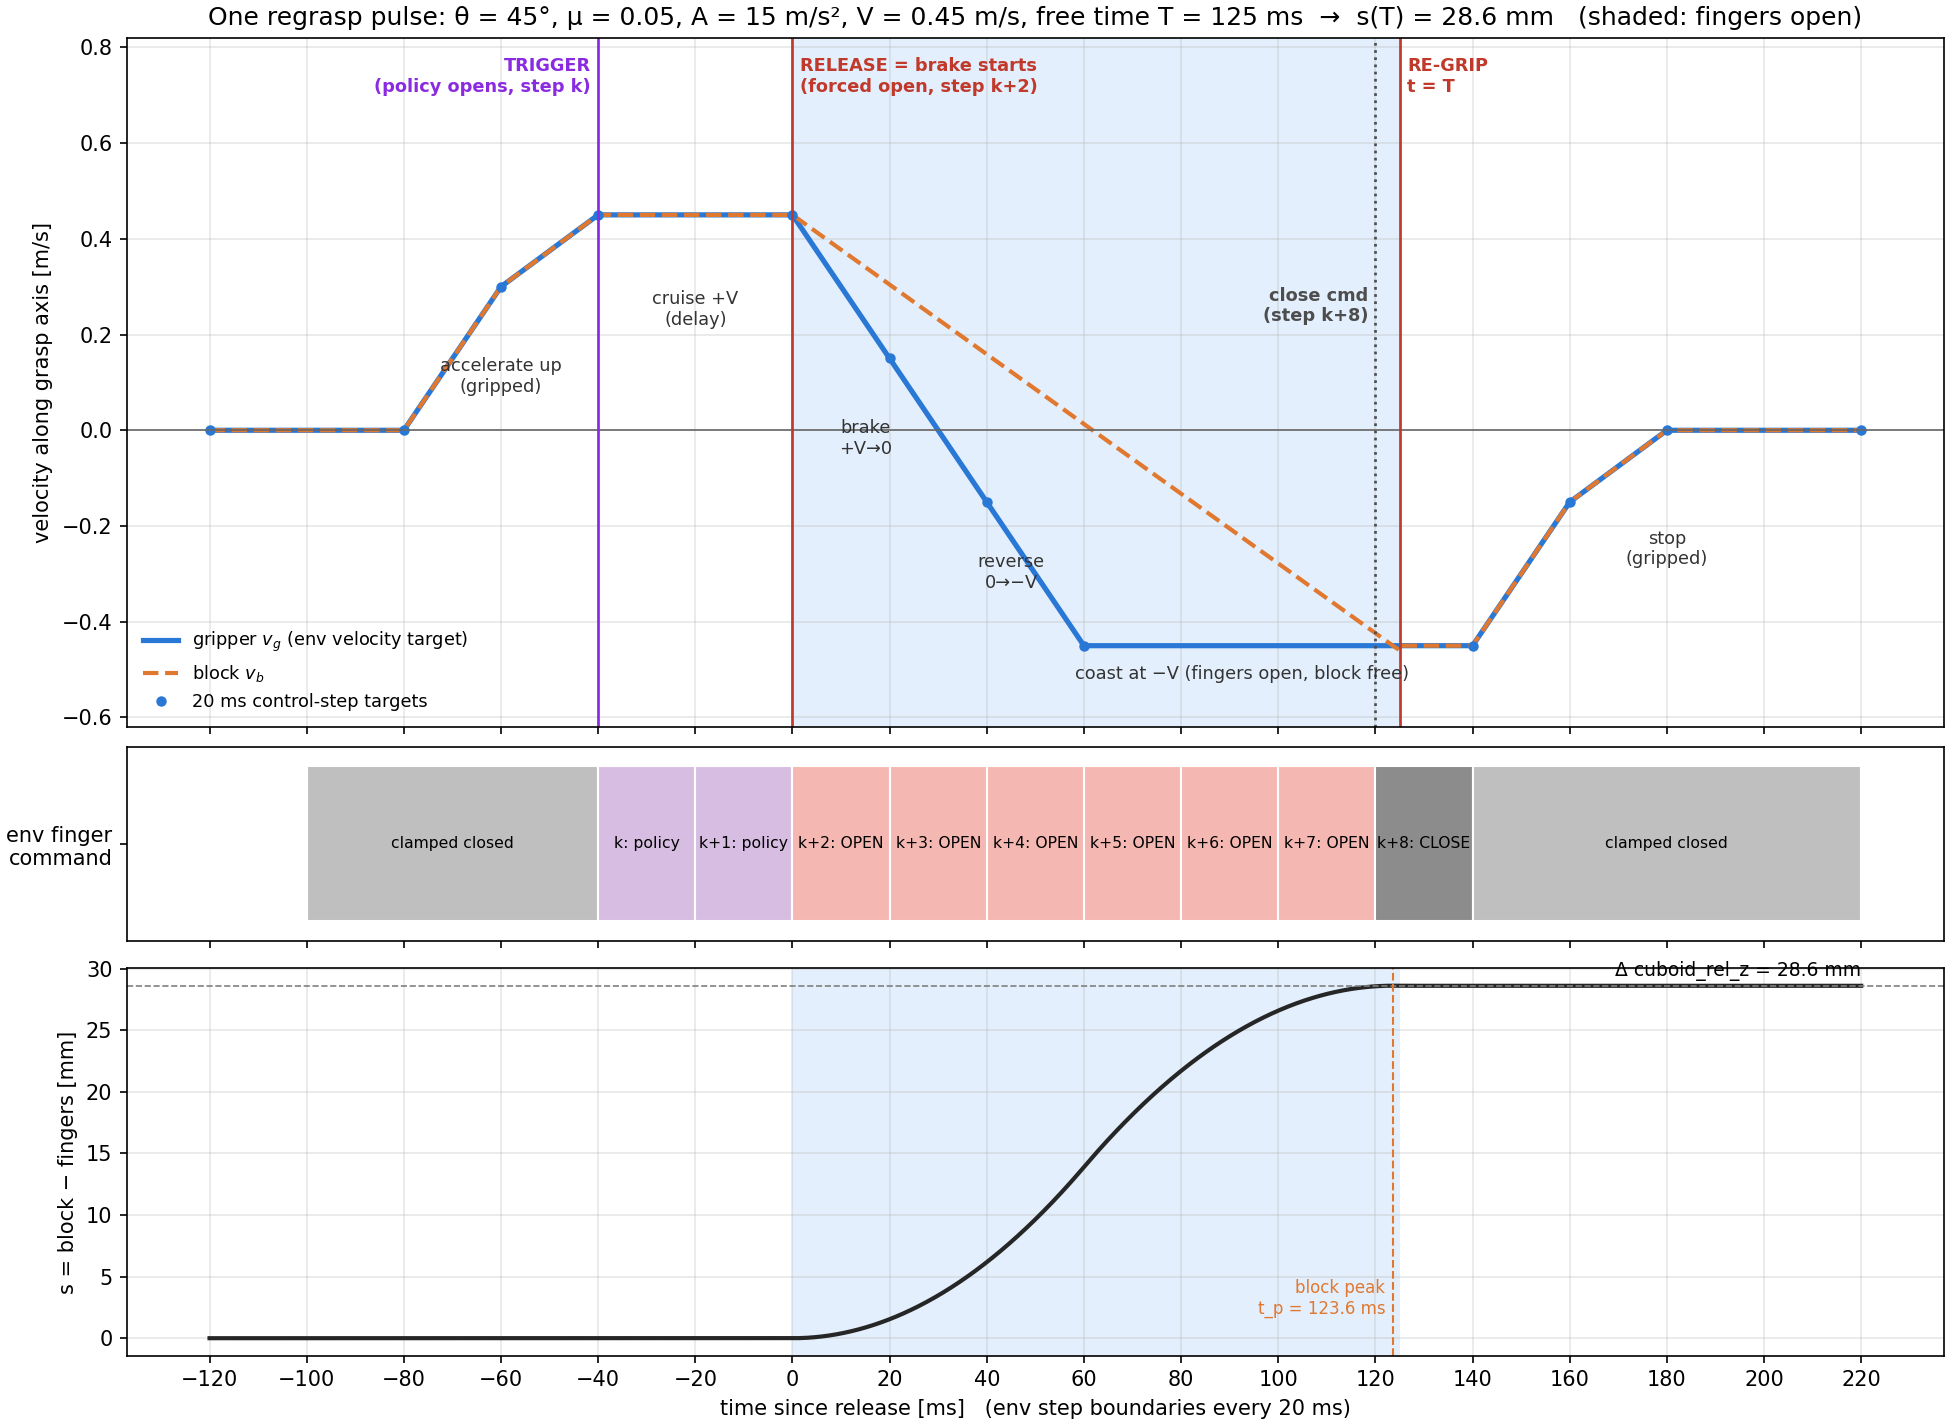
\includegraphics[width=\linewidth]{fig_timeline.png}
  \caption{One pulse for $\theta=45^\circ$, $\mu=0.05$, $A=15$\,m/s$^2$, $V=0.45$\,m/s, $T=125$\,ms. Top: gripper
  (blue) and block (orange) velocity along the axis. They coincide while gripped and separate in the shaded open
  window. The area between them is the regrasp. Middle: the env's finger command per 20\,ms step, relative to the
  trigger step $k$. Bottom: the block's displacement in the fingers, which ends at $+28.6$\,mm.}
  \label{fig:timeline}
\end{figure}
